%PART_2_CHAP_3
\myChapter{A}{ctivités et séquences pédagogiques}\label{sec:activite}
%WAIT a Review ok
\begin{resumChap}
Après avoir défini le matériel spécifique à disposition dans notre Kit robotique, nous aborderons dans ce troisième chapitre le cœur de ce qui constitue l'aspect pédagogique de ce kit: les activités.\par%
En premier lieu, nous discuterons du format à privilégier pour ces activités, à savoir: la temporalité de la séance, le support de la ressource ou encore la répartition des élèves. À cela, nous ajouterons certains éléments en rapport avec la scénarisation de l'activité, puis nous présenterons différents exemples:\par%
Nous présenterons les proto-activités qui avaient été désignées pour les premiers enseignants partenaires du projet; les projets d'élèves qui en ont découlé; puis la formalisation de ce travail au travers du livret pédagogique. Enfin nous présenterons une série d'activités \cro{clé en main} tant dans le langage de programmation visuel \sht{snap} que dans le langage Python.\par%
En dernier lieu, nous présenterons d'autres activités ayant eu lieu avec les robots humanoïdes et qui illustrent la diversité des projets potentiellement réalisables.\par%
Un point sur les limites de mise en place de ces projets sera également effectué.
\end{resumChap}{}
\myPhantom{paragraph}{Introduction}
    Au-delà des logiciels et matériels décrits dans le chapitre précédent, le kit robotique ErgoJr comprend également des activités pédagogiques. Elles ont également été co-créées avec les enseignants et mises à disposition en licence libre open source pour être utilisées telles quelles, ou en version modifiée, ou encore pour simplement servir de sources d'inspiration.\par%
    Pour la construction d’activités pédagogiques autour du robot PoppyJr, nous avons fait le choix de privilégier une approche coopérative~\citeB{kim2015robotics}: les élèves travaillent par groupe de deux ou trois et l’enseignant est là pour les accompagner, les guider dans leurs questionnements (quand c’est nécessaire), et faciliter les interactions. Les élèves travaillent donc en collaboration~\citeS{sec:user_cible} et de façon autonome en découvrant, en expérimentant, par le biais d’une démarche d’investigation. Au sein de cette démarche, l’erreur est perçue comme un élément essentiel de l’apprentissage~\citeS{sec:erreur}, et permet la construction de la connaissance. L’objectif est que l’élève manipule, qu’il mette en œuvre les ressources nécessaires à son apprentissage dans le but de produire des solutions à une problématique~\citeS{sec:tangible}.
    Les membres de l’équipe Poppy Education se sont donc mobilisés pour construire des activités pédagogiques correspondant à l’ensemble de ces principes et dans le respect des objectifs pédagogiques. %Chaque activité a été construite selon une grille standardisée. 
    L’objectif était également de proposer des activités pédagogiques plaisantes, mobilisant les compétences de l’élève de façon transversale~\citeS{sec:pluri_bot}, faisant appel à sa créativité, optimisant sa motivation et proposant un niveau de difficulté adapté (suffisamment élevé pour que l’activité soit stimulante tout en restant à la portée de l’élève~\citeF{fig:FlowModel}. Il était donc essentiel de prendre en compte, notamment, l’accessibilité pour les deux genres, les différences interculturelles, l’hétérogénéité des élèves, le développement durable (enjeux de long terme) ainsi qu’un esprit coopératif. Plusieurs éléments nous ont guidé dans cette construction~\citeB{toffoli2010analyse}.
\section{Formats et objectifs}
    \subsection{Répartitions}
        \paragraph{TD \& CM} 
            Les deux modes de répartition que l'on retrouve traditionnellement dans les établissements scolaires sont les \sht{CM} ou les \sht{TD}. Ces deux modes ont leurs avantages et sont souvent utilisés alternativement par les enseignants. Généralement, les \sht{CM} sont propices à la présentation des objectifs, la mise en place d'une séquence, ou, en milieu ou fin de séquence, ils sont propices à la généralisation des concepts manipulés précédemment et à fournir des conventions de nommage. En revanche, les \sht{TD}, eux, sont propices à la manipulation, l'exploration, la découverte tangible d'un phénomène (même abstrait), ils peuvent donc intervenir en tant que prémices, en tant que illustration ou en tant que mise en pratique. Ces deux modes ont été explorés dans certaines de nos activités  \cro{clé en main} (notamment car elles ont été co-dévellopées avec les enseignants); mais il est également possible de déconstruire les différents éléments des activités pour remonter un scénario correspondant aux besoins spécifiques de l'enseignant.
        \paragraph{Seul ou en groupe}
            Notamment il peut choisir de faire travailler ses élèves, seuls, ou en groupe, ou d'alterner ces deux modes, suivant ses objectifs théoriques et pédagogiques: il est parfois préférable de faire travailler individuellement des élèves sur une ou plusieurs compétences bien particulières (personnalisées à l'élève) pour, par exemple, combler un retard ou un décalage par rapport au groupe ou encore pour s'assurer qu'une compétence est bien acquise pour l'ensemble des élèves d'un groupe, \etc. 
        \paragraph{Fiche guide \& projet ouvert}
            Il peut également développer ses propres fiches guide ou encore définir des projets libres (\eg où les élèves établissent l'objectif \etou le cahier des charges répondant à cet objectif). Ce type de configuration est particulièrement bien adapté à la robotique, puisqu'il y a un besoin de compétences et spécialisations multiples rarement présent chez un seul individu, il y a donc un réel avantage au travail de groupe. De plus, l'autonomie et le contrôle conféré ainsi à l'élève impactent son investissement (sa motivation). C'est d'ailleurs le choix qu'a fait la majorité des enseignants de \sht{ICN} \& \sht{ISN} après quelques séances d'initiations~\citeS{sec:entretiens}.
    \subsection{Supports \& matériel}\label{sec:support}
        \paragraph{L'attention divisée}
            L'utilisation d'un robot dans une activité divise l'attention. En effet, l'utilisateur programmant le robot, doit alterner entre deux éléments de son environnement: la zone de programmation et le robot. À cela s'ajoutent plusieurs distracteurs durant la réalisation du \sht{TD} ou projet: ses camarades et l'enseignant. De plus, avoir une activité ou un projet implique d'avoir une fiche guide ou un cahier des charges. Ainsi, quatre \textit{spots} attentionnels sont à prendre en considération: \Li les actions du robot \ii la rédaction du programme \iii le suivi de la fiche guide \iiii les interactions sociales. 
        \paragraph{Le papiers}
            Ainsi, comme il convient de situer localement ces différents spots et de leur attribuer une charge modale différente, nous avons choisi d'éditer nos fiches guides (ainsi que le livret pédagogique fourni dans le kit ErgoJr) sur papier et d'inciter à imprimer ces ressources plutôt que d'exploiter leur version pdf. Ceci car, dans ces circonstances, il y aura superposition des modalités; voir des supports, si un seul ordinateur est disponible pour le groupe, et typiquement, le \sht{pdf} et l'interface de programmation, ne pourront pas être affichés simultanément. Dans tous les cas, pour réaliser l'activité, les étudiants devront partager les ressources (efficacement) s'ils travaillent en groupe.
        \paragraph{Les ressources}
            Tous les établissements, et tous les enseignants ne sont pas équivalents. Ainsi, certains sont équipés et à l'aise avec de nombreuses plateformes accumulées, parfois, depuis de nombreuses années grâce, par exemple, aux cours de  \cro{technologie} qui ont toujours été particulièrement s à ce type de détournement, ou via des clubs de robotique sur des temps péri-scolaires.
            \subparagraph{Additionnelles}
                Certaines classes ont donc du matériel supplémentaire à disposition, qu'ils vont pouvoir étudier, comparer et sélectionner suivant leurs besoins et créer des projets très atypiques ou ambitieux et parfois qui le sont trop et qui provoquent une certaine frustration.
            \subparagraph{En manque}
                Mais cette frustration peut naître également d'un manque de ressources ou de matériel à disposition pour mener à bien leurs projets. Ou dans le cadre d'activités plus cadrées, comme des \sht{TD}, être soumis aux bugs et autres  \cro{caprices} du réseaux de l'établissement n'autorisant pas \tiret{par moment} certaines manipulations\dots
    \subsection{Temporalité}
        \paragraph{Multiples séances}
            C'est bien sûr le choix le plus commun chez les enseignants: étant donné, d'une part, qu'ils souhaitent rentabiliser l'investissement matériel (\eg l'utiliser) et d'autre part, car il semble naturel de construire une séquence pédagogique sur plusieurs séances permettant ainsi à l'élève d'avoir du temps de recul et d'atténuation, permettant une bonne mémorisation des connaissances à long terme. Cependant, même si l'objectif global se porte sur un cheminement de plusieurs séances, chacune des séances composant ce parcours peut être perçue comme une séance autonome. De plus, certains enseignants, novices en robotique, peuvent avoir le besoin de tester certaines activités de découverte en amont.
        \paragraph{Séance de découverte et de prise en mains}
            Nous avons développé plusieurs activités de prise en main et de découverte du robot qui permettent à un individu totalement novice en programmation (et robotique) d'apprendre en quelques heures (une séance) à contrôler les fonctions élémentaires du robot pour réaliser un défi \eg  \cro{le chamboule-tout}~\citeS{sec:livret}.
        \paragraph{D'autres contextes}
            Ces activités de découverte, et d'autres~\citeS{sec:handKey}, ont notamment été développées et testées dans divers contextes tels que des stands à des conférences ou des workshops et des ateliers sur des salons ou des forums.
    \subsection{Apprentissage Programmation \& Robotique}
        \paragraph{Les notions}
            Comprendre les concepts élémentaires de l'informatique~\citeS{sec:concept}, ainsi que les notions permettant d'appréhender les différents types de paradigmes de programmation~\citeS{sec:program-concept} est un des objectifs essentiel des filières numériques. À cela s'ajoute les notions typiques de la robotique~\citeS{sec:bot-concept} et plus généralement au numérique~\citeS{sec:num-concept} et au autres domaines associés.%~\citeS{sec:link-concept}.
            Bien sûr, dans nos ressources, nous nous sommes davantage focalisés sur les notions inhérentes à la robotique \eg capteur, actionnaire, \sht{BSM}~\citeS{sec:handKey}.
        \paragraph{L'histoire}
            Dans les ressources que nous avons développées, nous avons toujours cherché à donner un objectif concret et proposer un défi: un problème à résoudre autour d'une histoire~\citeS{sec:storitell}. Et même si parfois la métaphore ou la comparaison peut sembler alambiquée (\eg ErgoJr se transforme en poule ou en caméléon), il semble qu'elle a surtout tendance à attiser l'étonnement et la curiosité, suscitant ainsi débat et motivation à prouver (ou infirmer) telle ou telle affirmation. Ce type d'échange, si correctement canalisé par l'enseignant, semble particulièrement bénéfique à la compréhension, la généralisation et la mémorisation des notions ainsi débattues entre pairs. Ceci est certainement induit par l'autonomie et le contrôle laissés à l'élève durant ce type d'échange~\citeS{sec:motiv}. Ainsi, le choix et la mise en scène de la séquence pédagogique doit aller au-delà de la simple illustration (\eg le traditionnel problème de mathématique \gui{un train part à $x$ heurs de la gare A \dots \etc}) qui n'apporte que peu de valeur pédagogique.
\section{Exemples d'activités}
    \subsection{En classe}
        \subsubsection{Proto-activités}\label{sec:proto-act}
            Lors de la phase de conception de base de 10~propositions d'activités aux enseignants~\citeS{sec:ucd_prop}, ils étaient totalement libres de les utiliser en l'état ou de les modifier. Ils pouvaient également laisser ce choix aux élèves. Chacun des enseignants a adapté les projets en fonction de leurs compétences initiales, donnant une grande variété de projets. Parmi les projets réalisés, 7~permettent d'illustrer une grande partie des usages rencontrés dans ces lycées:
            Deux projets basés sur des activités proposées;  \cro{Garçon de café}~\citeURL{LV-cafe} dérivé de l'activité  \cro{robot vs automate} est une activité où l'on commence par coder le mouvement d'un automate: déplace la pince, ferme la pince, \etc; puis l'on ajoute un capteur: si j'attrape quelque chose, alors je me déplace, le comportement s'adapte alors à la présence ou non du sucre. Le but était ici d'amener à la notion et la définition de robot. 
            L'activité  \cro{serveur au tennis de table}~\citeURL{YB-basket} reprend l'activité  \cro{chamboule tout}~\citeURL{PE-chamboule} qui consiste à se servir du robot comme d'une catapulte. Ici l'intérêt est d'aborder des notions de mathématiques et de physique (\eg angle, trajectoire, vitesse, \etc). 
            Deux projets basés sur le traitement de l'image: trieur de couleurs et trieur de conteneurs. Dans le premier, il fallait utiliser un robot et sa caméra pour détecter la couleur d'une balle, les instructions étaient envoyées à un second robot se chargeant de déplacer la balle dans la bonne boîte~\citeURL{YB-triColors}. Le second projet était similaire: dans une reproduction du port de Rotterdam~\citeURL{SS-Rotterdam}, un robot devait en fonction du QRcode, inscrit sur le conteneur, le trier.
            Enfin le projet  \cro{tic-tac-toe}~\citeURL{PE-tictactoe} initialement proposé par l'équipe s'est vu largement détourné. Les enseignants ont d'abord conçu et réalisé les projets chez eux, puis, suivant les notions qu'ils souhaitaient aborder avec leurs élèves, ils ont fourni un certain nombre d'éléments de réflexion. Ainsi dans un premier projet, les élèves ont principalement travaillé sur le traitement de l'image via une webcam externe en processing~\citeURL{CC-tictactoe}. Dans le second projet, la connectivité était le point focal, ici le traitement de l'image (pour connaître la position des pions sur la grille) a été remplacé par l'ajout de photorecepteurs sous la grille grâce à une carte arduino programmable en \sht{snap}~\citeURL{GL-tictactoe}. Le troisième projet s'est plutôt concentré sur la théorie des jeux et sur comment créer de l'aléatoire dans un langage de programmation, ici la plateforme robot n'était présente que comme support illustrant les codes réalisés par les élèves.
        \subsubsection{Projets d'élèves}
            Les enseignants et les élèves ont créé et réalisé des activités et projets qui s'inscrivent généralement dans la continuité du livret pédagogique (apportant les pré-requis nécessaires~\citeS{sec:livret}). Ci-dessous sont présentés une séquence d'activité de seconde \sht{ICN} et un projet de terminale \sht{ISN} créés par deux enseignants partenaires et réalisés avec leurs élèves; d'autres activités issues directement des enseignants seront présentées plus loin~\citeS{sec:entretiens}.
            \paragraph{ErgoJr Marin, OhéOhé}
                Lors de la deuxième année d'utilisation des robots, un enseignant nous a présenté cette activité presque finalisée en nous demandant un conseil technique (pour faire communiquer, en \sht{snap}, deux robots entre eux). Une fois l'activité réalisée, il nous a envoyé toutes ses ressources en vrac pour qu'on puisse la documenter et la partager~\citeURL{LV-marin}. Les élèves ont également produit une vidéo explicative~\citeURL{LV-marin-video}. 
                L'objectif de cette séquence est de programmer deux robots pour qu'ils échangent des messages en langage sémaphore, entre deux points de la classe. Une fiche d’activité guide les élèves au cours des 12 séances.
                Concernant les objectifs pédagogiques mis en jeu dans cette activité: en binôme, les élèves apprennent à construire et programmer un dispositif robotique en respectant un protocole précis (le langage sémaphore). Ils acquièrent les compétences nécessaires pour lire, comprendre un programme pour être capable de le modifier. Les notions de base en programmation telles que les fonctions, fonctions input(), listes, variables et boucles sont abordées. 
                \begin{figure}[!h]
                  \centering
                  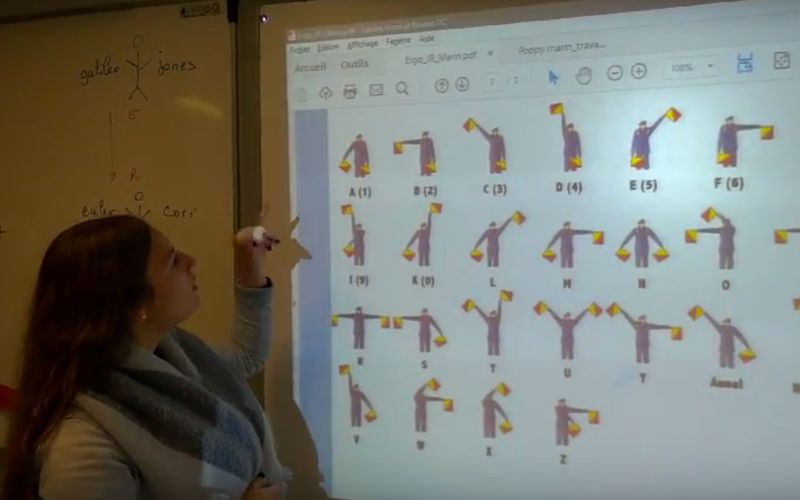
\includegraphics[width=0.49\linewidth]{Figures/Noirpoudre-Semaphore.png}
                  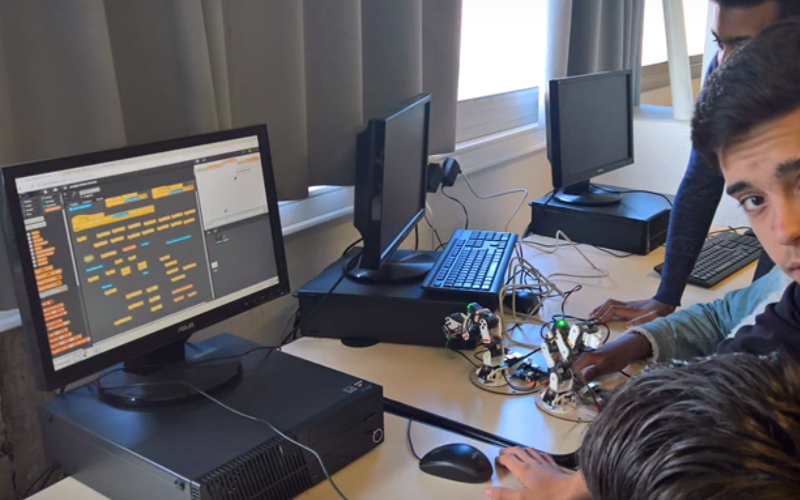
\includegraphics[width=0.49\linewidth]{Figures/Noirpoudre-semaphore_prog.png}
                  \caption{Réalisation du projet ErgoJr Marin}\label{fig:act_semaphore}
                \end{figure} 
            \paragraph{ErgoJr joue à TicTacToe}
                Ce projet de terminale\sht{ISN} vise à faire jouer le robot Poppy ErgoJr au TicTacToe contre un humain en utilisant la vision par ordinateur (caméra).
                Cette fois, l'enseignant s'est inspiré du projet TicTacToe~\citeURL{PE-tictactoe} pour se l'approprier, le réaliser et le proposer à un groupe d'élèves. Des échanges réguliers ont eu lieu au fur et à mesure de l'avancement du projet, notamment sur le forum, lors d'une réunion et lors de déplacements en salle de classe. De plus, un autre enseignant s'est inspiré de ces échanges, pour en faire une version adaptée à ses élèves de seconde\sht{ICN}~\citeURL{CC-tictactoe}.
                \begin{figure}[!h]
                    \centering
                    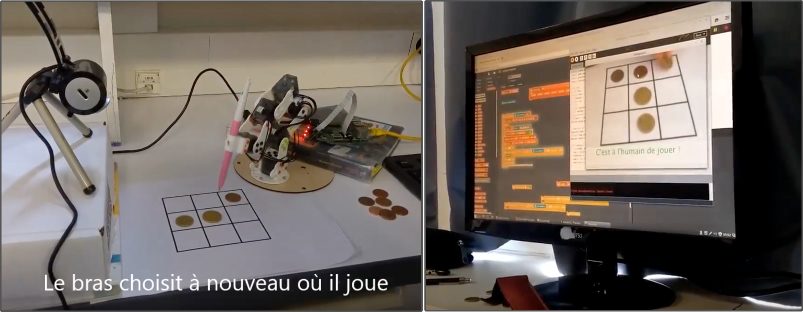
\includegraphics[width=\linewidth]{Figures/Noirpoudre-tic-tac-toe.png}
                    \caption{Activité Tic-tac-toe}\label{fig:tic-tac-toe}
                \end{figure}\par%
                Ce projet \sht{ISN}, réalisé par un groupe de trois élèves, permet à la fois une introduction à la théorie des jeux et à la robotique en créant un système de développement robotique (action et vision: Poppy ErgoJr + Raspberry~Pi + \sht{snap} + Webcam) en interaction avec l'environnement et une résolution et programmation d'un problème ouvert en implantant des fonctionnalités avec \sht{snap} et Processing (langage de programmation proche de Java), en faisant communiquer les applications (inter-langage) à l'aide d'un serveur web, et en s'initiant à l'analyse d'image et à la vision par ordinateur. 
                Par ailleurs, les élèves ont utilisé les ressources mises à disposition par la plateforme Poppy, en cherchant des informations sur le forum et la documentation et en tenant
                un journal de bord sur le forum pour présenter leur progression séance par séance~\citeURL{CC-tictactoe}.
    \subsection{Découverte avec le livret}\label{sec:livret}
        La première activité du livret (Contrôler Poppy ErgoJr~\citeURL{PE-chamboule}) apprend à faire bouger le robot en \sht{snap} afin d'apporter les notions nécessaires pour réaliser le défi \textit{ErgoJr joue\dots chamboule-tout: quelle est la meilleure manière de lancer la balle ?} visant à contrôler la position et la vitesse des moteurs du robot pour lancer la balle et faire tomber l’empilement de gobelets. Les retours des utilisateurs ont été essentiels afin de permettre de la simplifier et de cibler les priorités. Ce défi a pour origine une des premières démonstrations que l'équipe Poppy Education a présenté lors de salons à destination des enseignants et du grand public. Nous avions alors remarqué que ce programme très simple et amusant~\citeURL{PE-chamboule-demo} attisait la curiosité et était une bonne accroche pour présenter d'autres choses.\par%
        Conformément au programme\sht{ICN}~\citeF{fig:Chamboule_tout}, les élèves doivent résoudre un problème et le programmer, ainsi que développer des compétences annexes.
        Concrètement, en situation réelle, on observe qu'en deux heures, les groupes de trois ou quatre élèves sont capables de programmer des mouvements simples et de proposer une solution au problème. Il n'y a aucun groupe en échec et les plus avancés complexifient même leur programme, explorent d'autres manières de lancer la balle et se lancent eux-mêmes des défis (comme faire rebondir la balle au-dessus d'un verre avant d'atteindre l’empilement de gobelets). Plus précisément, les élèves collaborent, échangent des idées, se mettent d'accord sur un mouvement à effectuer pour résoudre le problème et sur le programme à réaliser pour vérifier leur hypothèse. Puis, ils lancent leur programme et observent le résultat. Finalement, ils mobilisent leur esprit critique et utilisent les informations que fournit le robot pour améliorer le programme, tout en exprimant leur créativité.
        \begin{figure}[!h]
            \centering
            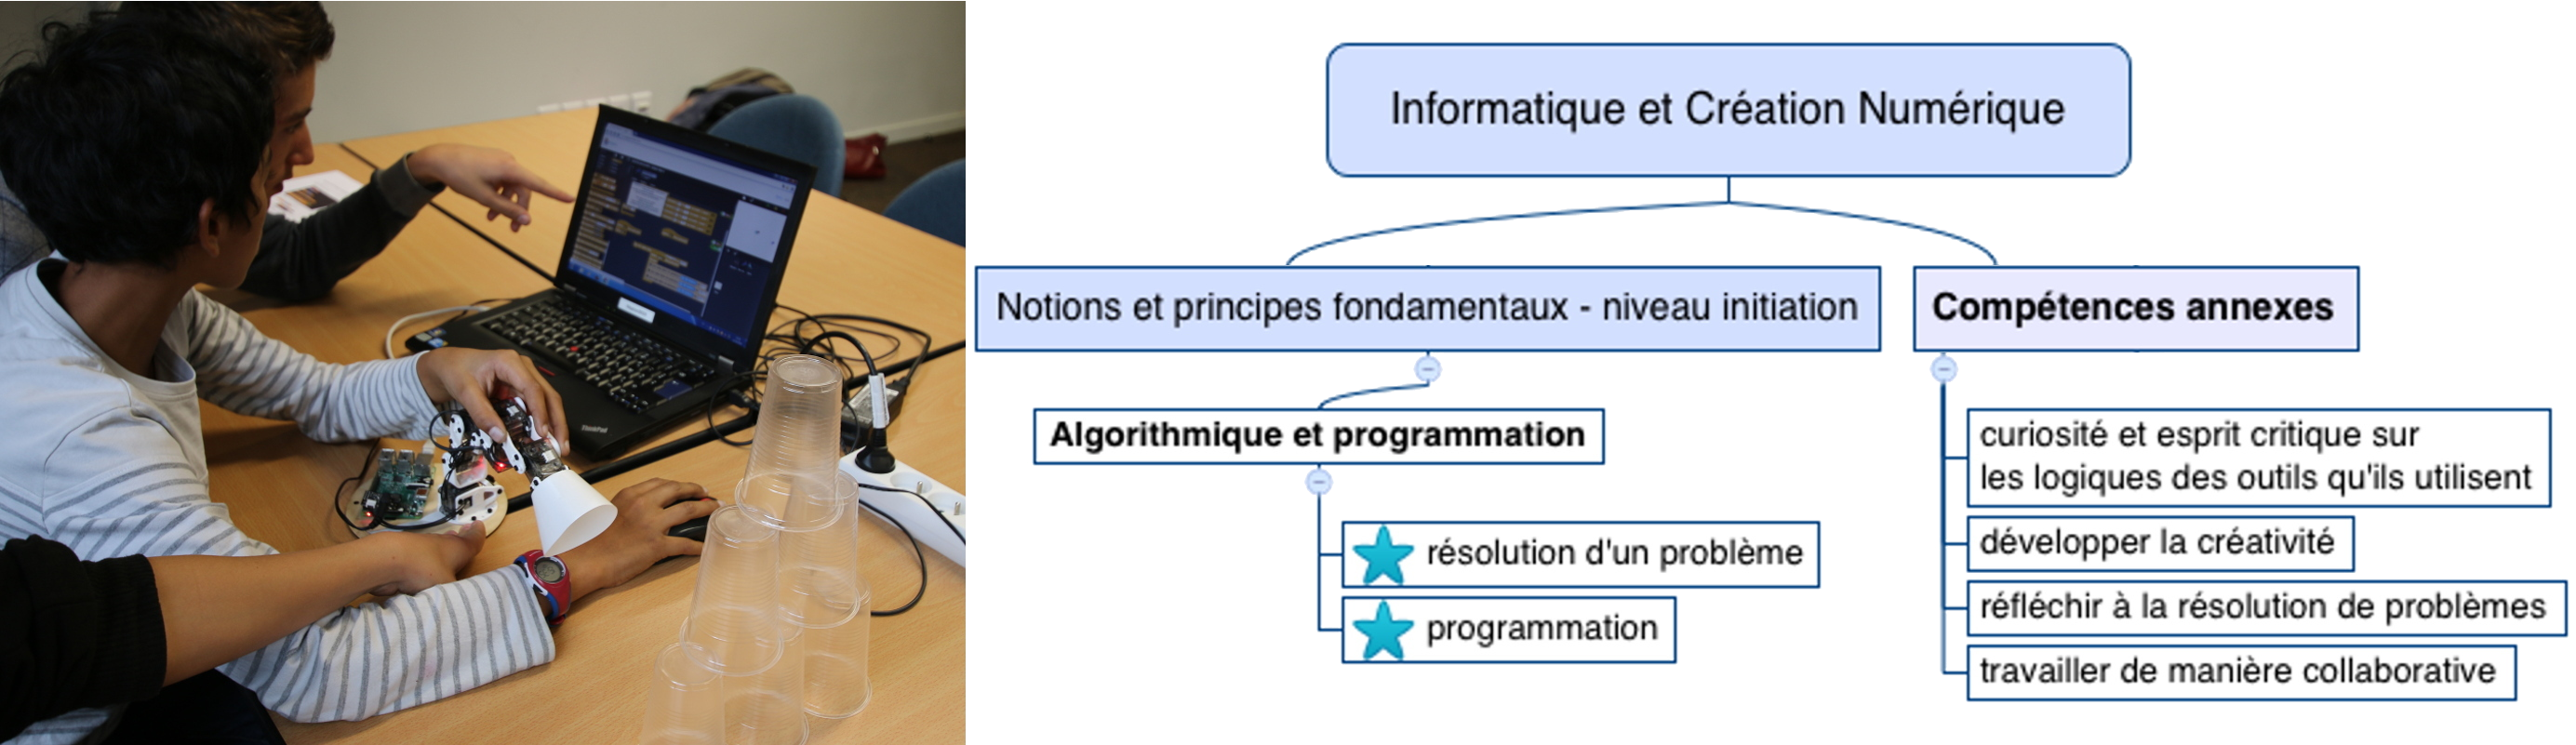
\includegraphics[width=\linewidth]{Figures/Noirpoudre-chamboule-tout.png}
            \caption{Liens avec le programme d'ICN pour l'activité Chamboule-tout, Noirpoudre~\cite{RI}}\label{fig:Chamboule_tout}
        \end{figure}\par%
        Il est important de souligner que l'activité et le robot ne suffisent pas en eux-mêmes, l'enseignant, en tant qu'expert en pédagogie et connaissant ses élèves, joue un rôle primordial dans l'accompagnement de ces apprentissages (pour prendre du temps, pour faire un point sur les notions vues, expliciter des étapes, \etc) et pour tirer parti des bénéfices du travail de groupe (aider les élèves à s'organiser, échanger les rôles, \etc). En effet, comme le souligne cet enseignant de seconde, qui dans son compte-rendu~\citeURL{SP-cr}, a l'impression qu'en autonomie, certains élèves  \cro{font pour faire} et n'adoptent pas automatiquement les bonnes démarches pour acquérir les notions visées (ce qui demande d'être actif cognitivement).
    \subsection{Activités clé en main}\label{sec:handKey}
        Ces activités sont construites sur des formats courts (une séance de 2~à 3h) et ne suppose aucune connaissance préalable, tant en programmation qu'en robotique: le niveau de difficulté augmentant progressivement; de plus elle s'adapte aussi bien à des utilisateurs adultes (dans le cadre de formation) ou mineurs (dans le cadre de la classe). D'autres modules sont proposés en tant d'exhibition. 
        \subsubsection{En \textit{Snap!}}
            \paragraph{Préambule}
                Ces activités ne nécessitant pas de connaissances préalables, il était nécessaire dans un premier temps de familiariser l'utilisateur avec l'interface de \sht{snap}. En effet, certains éléments peuvent paraître trompeurs \eg certains blocs servant à déplacer le  \cro{sprite} pouvant être pris pour des blocs déplaçant le robot. De plus, certaines formes, certaines couleurs possèdent une signification propre (qui pourront générer des affordances une fois acquises). Ainsi, nous avons développé une activité courte (1~page) qui permet de mettre rapidement en lumière ces différentes significations et de distinguer facilement les éléments relevant du contrôle du robot à ceux relevant du contrôle interne à \sht{snap}. Cette phase d'appropriation des spécificités de \sht{snap} est visible en préambule des activités  \cro{poule}~\citeA{pdf:act_poule} et  \cro{caméléon}~\citeA{pdf:act_cameleon}. Durant cette phase sont également introduits des éléments de base de programmation qui seront nécessaires pour réaliser l'activité, à savoir, les variables, les boucles et les conditions. Les notions sont présentées de manière implicite sous forme de petites questions pouvant paraître triviales, mais qui relèvent d'une certaine complexité pour des utilisateurs non habitués à ce type de formulation.
            \paragraph{Chamboule tout}
                Cette activité a pour objectif de permettre à l'utilisateur de prendre en main rapidement et facilement les fonctionnalités de base du robot autour d'un défi ludique~\citeA{pdf:act_chamboul}. 
                \begin{figure}[!h]
                    \centering
                    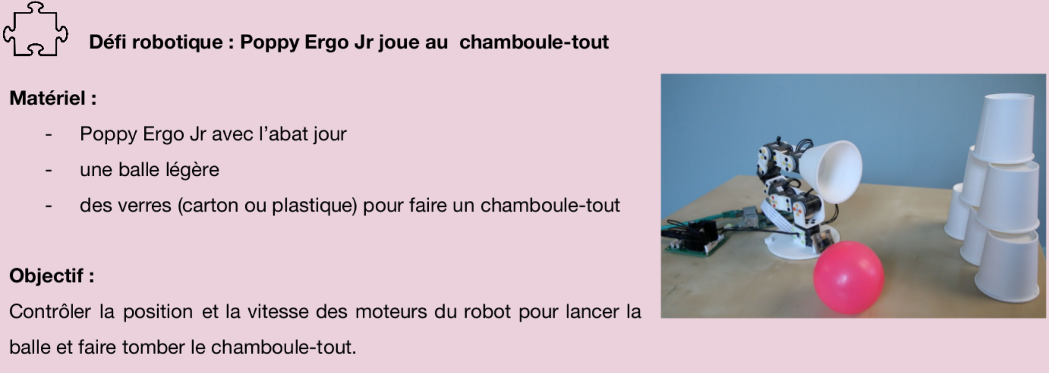
\includegraphics[width=0.8\linewidth]{Figures/Desprez-act_chamboule.png}
                    \caption{Défi Chamboule-tout}\label{fig:act_chamboule}
                \end{figure}\par%
                Cette activité initialement créée pour répondre aux besoins du programme de \sht{ICN}~\citeF{fig:Chamboule_tout} s'est trouvée particulièrement efficace dans de nombreuses situations pour faire découvrir le robot. C'est par ailleurs l'une des premières activités qui a été développée et elle se retrouve également dans le livret pédagogique.
            \paragraph{Caméléon}
                Cette activité~\citeA{pdf:act_cameleon} a pour vocation de faire découvrir la caméra sous un autre angle: ici elle sert de capteur de couleurs, qu'il faut calibrer, puis associer à une action, ici allumer les leds des moteurs dans la couleur détectée.
                \begin{figure}[!h]
                    \centering
                    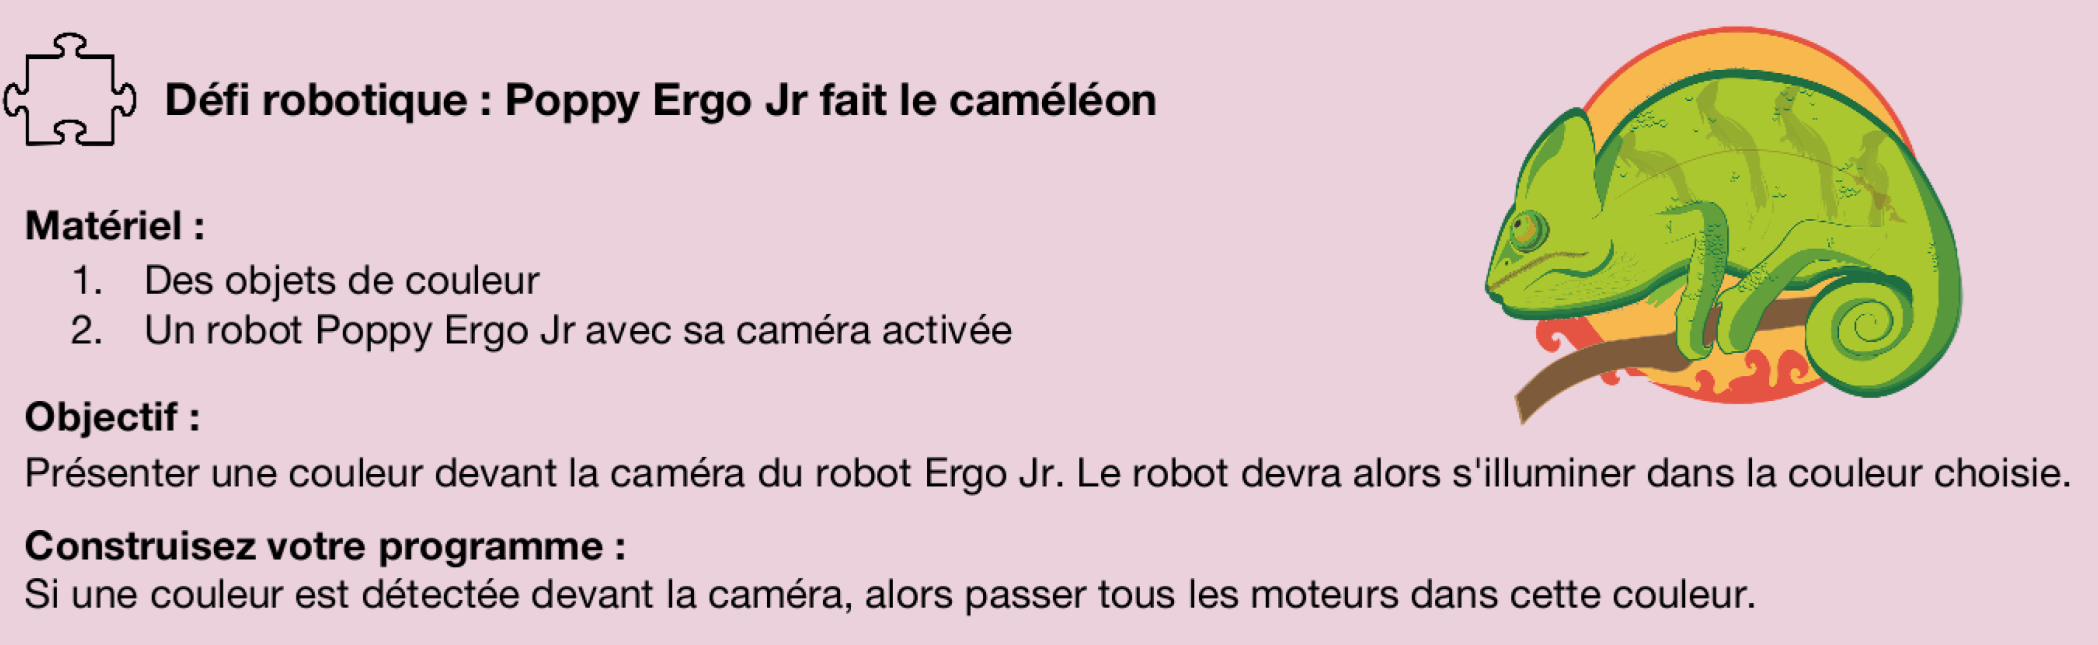
\includegraphics[width=0.8\linewidth]{Figures/Desprez-act_cameleon.png}
                    \caption{Défi Caméléon}\label{fig:act_cameleon}
                \end{figure}\par%
                Dans un premier temps, il faut donc calibrer et détecter les couleurs, puis insérer une boucle conditionnelle au sein d'une boucle infinie, en précisant le jeu de couleurs et l'action associée.
                Cette activité est l'une des dernières réalisée par l'équipe notamment car elle réclame l'ajout de plusieurs blocs et les entrées dans l'\sht{api} correspondante~\citeURL{TS-bloc_color}.
            \paragraph{Poule}\label{sec:act_poule}
                L'objectif de cette activité~\citeA{pdf:act_poule} est de faire découvrir une notion commune à tout organisme dynamique placé dans un environnement: la \glsdesc{BSM}.
                Ici, le robot est composé de 6~moteurs redondants par paires sur 2~axes, il  \cro{suffit} de coupler les 3~moteurs inférieurs avec les 3~supérieurs, en appliquant une fonction négative~\citeF{fig:prog_poule}. Autrement dit, nous récupérons la position (en degrés) des 3~moteurs qui sont manipulés (mode \textit{compliant}), on multiplie alors ces valeurs par~$-1$, puis on envoie ces nouvelles valeurs aux 3~moteurs pilotés par \sht{snap} (mode \textit{stiff}). Pour arriver à cela, il faut donc s'assurer que les rudiments de programmation en \sht{snap} sont acquis par l'utilisateur, d'où la présence de la séquence préambule. Puis, l'utilisateur doit être en mesure de contrôler le robot: récupérer les informations des capteurs et envoyer des instructions aux effecteurs. Enfin, il doit comprendre l'objectif, le défi, et la consigne associée. Deux variantes ont été testées. 
                \begin{figure}[!h]
                    \centering
                    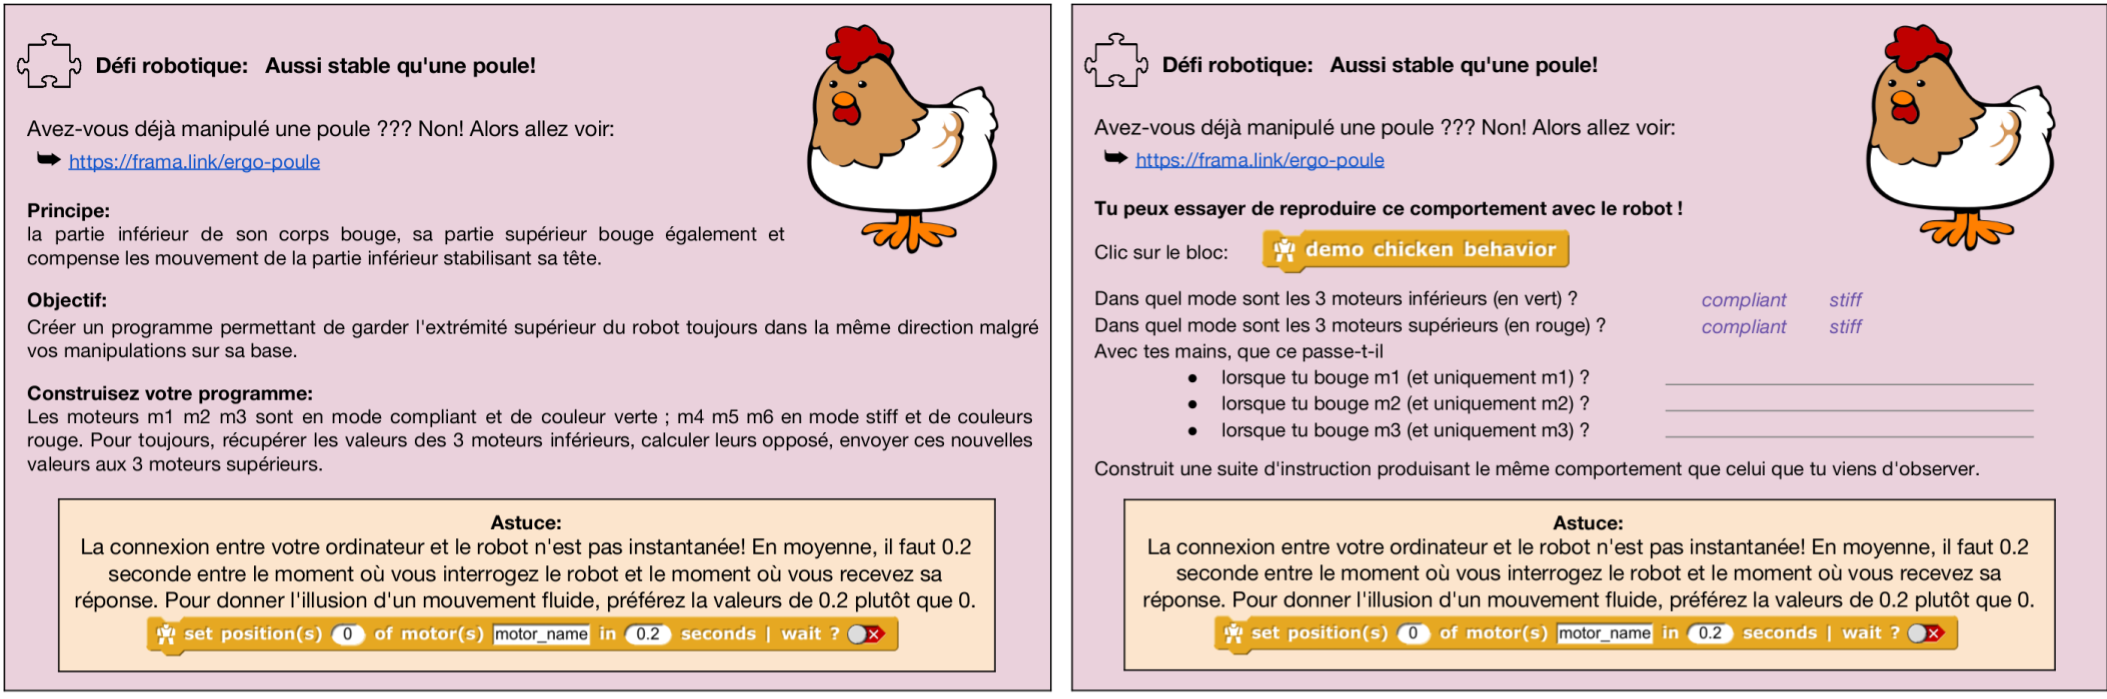
\includegraphics[width=\linewidth]{Figures/Desprez-act_poule.png}
                    \caption{Défi Poule - Deux variantes}\label{fig:act_poule}
                \end{figure}\par%
                Quand les étudiants arrivent à la quatrième page et commencent le  \cro{défi du poulet}, ils regardent d'abord une vidéo~\citeURL{TD-chicken-move} montrant l'action de la \sht{BSM} chez la poule pour stabiliser sa tête, puis une  \cro{modélisation} de son comportement sur le robot ErgoJr: c'est ce qu'ils ont à réaliser. Pour cela ils disposent des instructions suivantes:
                \gui{Les moteurs m1 m2 m3 sont en mode \textit{compliant} et de couleur verte; m4 m5 m6 en mode \textit{stiff} et de couleur rouge. Pour toujours, récupérer les valeurs des 3~moteurs inférieurs, calculer leurs opposés, envoyer ces nouvelles valeurs aux 3~moteurs supérieurs.}
                \begin{code}[!h]
                \begin{minipage}{\linewidth}
                    \subcaption{Solution \textit{Snap!}}\label{fig:prog_poule_snap}\par%
                    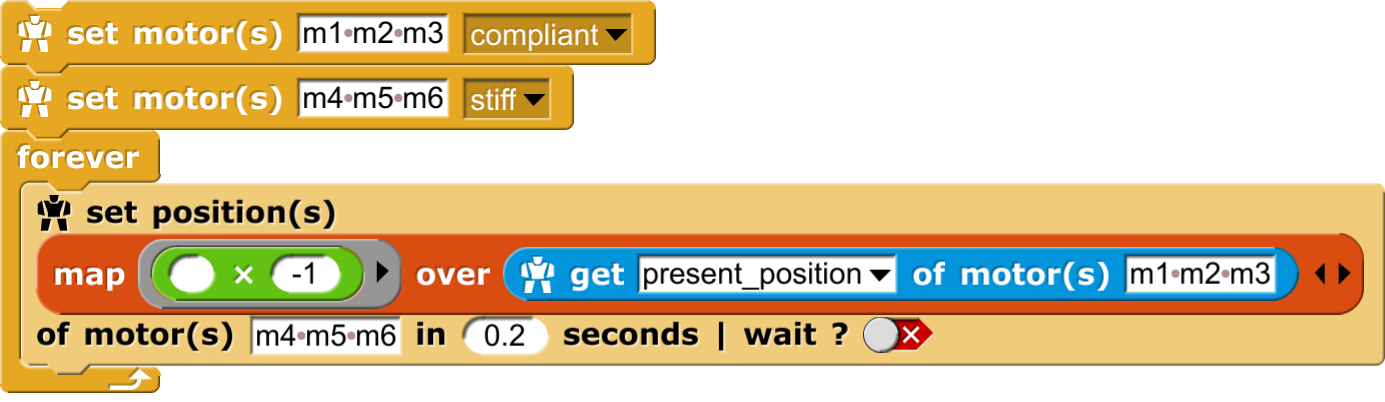
\includegraphics[width=0.8\linewidth]{Figures/prog-poule.png}
                \end{minipage}
                \begin{minipage}{\linewidth}
\subcaption{Solution python}\label{fig:prog_poule_python}
\begin{lstlisting}[language=Python,basicstyle=\footnotesize]
import time
from pypot.creatures import *
ergo= PoppyErgoJr()
for m in ergo.motors[0:2]:    m.compliant=False
for m in ergo.motors[3:5]:    m.compliant=True
while True:
    for i in range(3):
        ergo.motors[i+3].goto_position(
            (ergo.motors[i].present_position)*-1,
            0.1
        )
    time.sleep(0.01)
\end{lstlisting}
                \end{minipage}
                \vspace{-0.5cm}
                \caption[Défi Poule, solutions (\textit{Snap!} et python)]{Défi Poule, solutions}\label{fig:prog_poule}
                \end{code}\par%
                Dans la seconde version, quand les étudiants arrivent à la quatrième page et commencent le  \cro{défi du poulet}, ils regardent d'abord une vidéo~\citeURL{TD-chicken-move}, puis ils peuvent cliquer sur un bloc reproduisant le comportement observé dans la vidéo. Ils peuvent alors manipuler leur robot, le plier à droite, observer qu'il compense à gauche, \etc et tenter de comprendre ses actions et ses réactions. Ensuite, quelques questions sont posées pour mettre les étudiants sur la bonne voie: \gui{dans quel mode sont les moteurs verts / rouges?}, \gui{que se passe-t-il lorsque vous ne déplacez que le moteur m1 / m2 / m3?}. Les étudiants doivent comprendre ce que cela veut dire, inférer de ce qu'ils viennent d'apprendre et recréer ce comportement.
                Ces deux variantes ont été évaluées sur plusieurs aspects~\citeS{Exp:poule}.
            \paragraph{Boîte noire}
                Ce set d'activités a été développé pour offrir une première découverte avec le robot Poppy ErgoJr. Elle prend la forme d'un projet \sht{snap} accessible directement en ligne~\citeURL{TD-online}, et se compose de plusieurs  \cro{sprite} contenant chacun une démonstration différente:
                \subparagraph{Danse}
                    Propose d'enregistrer N positions puis de les rejouer dans l'ordre pour constituer une chorégraphie. Les valeurs en degrés de chaque moteur sont affichées, les positions sont modifiables ainsi que la vitesse.
                    \begin{code}[!h]                        \label{cod:prog_dance}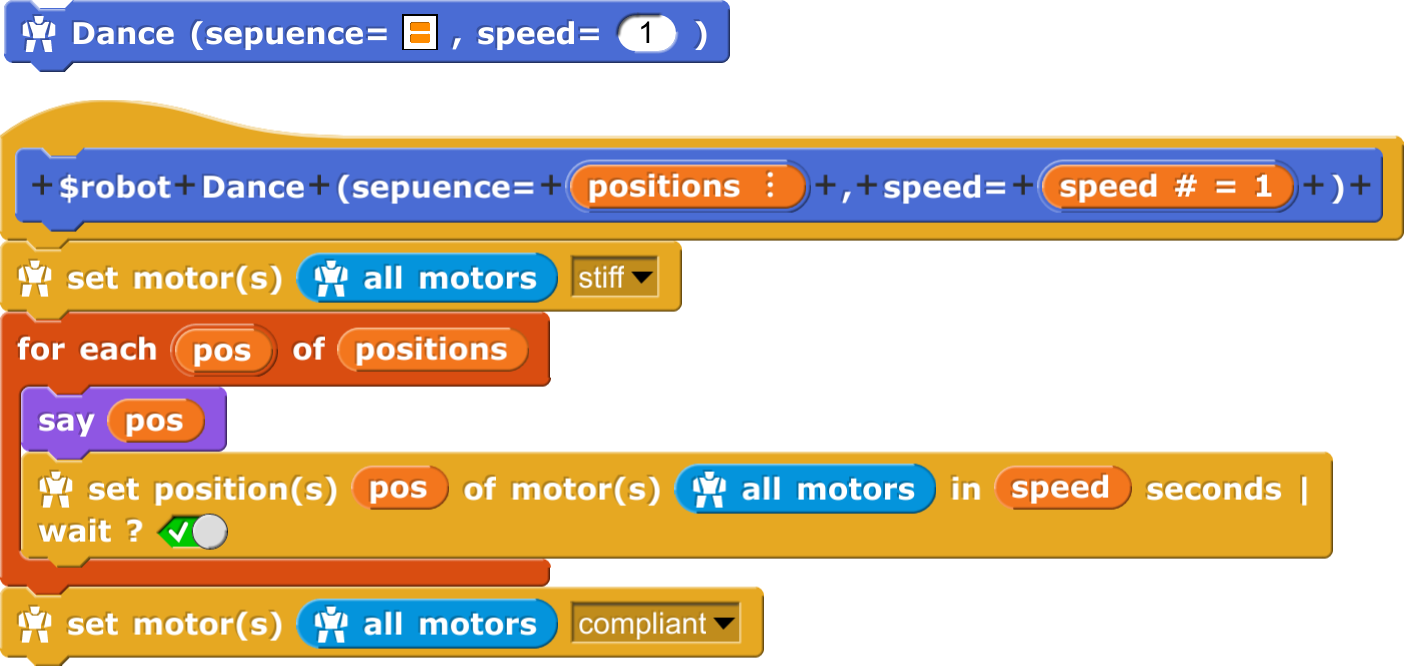
\includegraphics[width=0.9\linewidth]{Figures/prog-dance.png}
                        \caption{Bloc de démonstration - Danse}
                    \end{code}
                    Il est à noter que cette activité boîte noire est dérivée d'une activité~\citeA{pdf:act_dance} mise en œuvre lors d'une expérimentation pilote~\citeS{Exp:Reel_virtuel}. Cette activité proposait une série de photos du robot ErgoJr, l'utilisateur est invité à trouver la séquence de 6~valeurs qui permet de reproduire la posture arborée par le robot sur la photo.                \subparagraph{Chamboule-tout}
                    Propose d'enregistrer une position de départ, une position d'arrivée, de choisir une vitesse, pour faire tomber la tour!
                    \begin{comment}
                    \begin{code}[!h]                        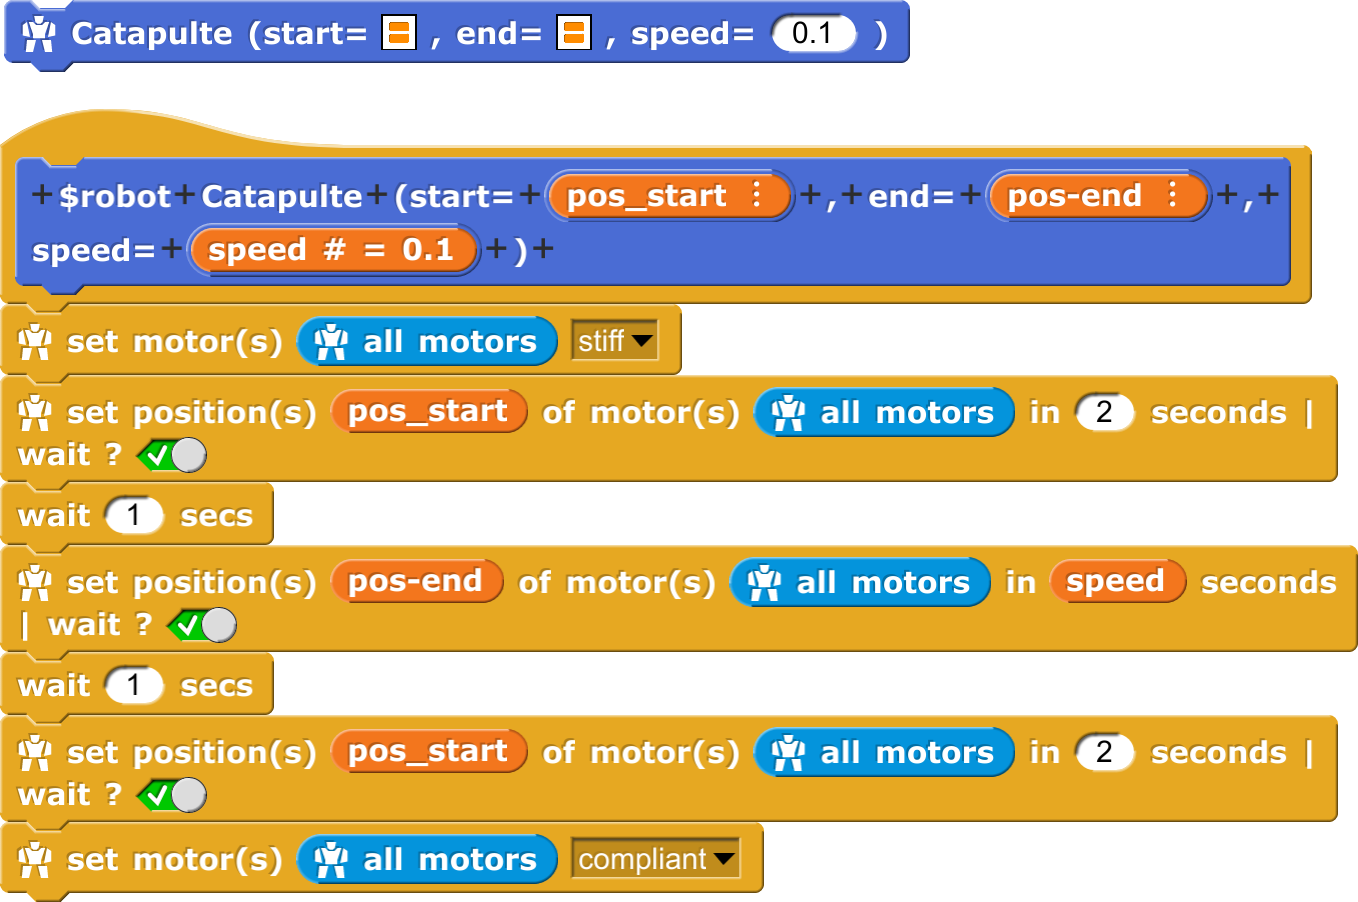
\includegraphics[width=0.9\linewidth]{Figures/prog-chamboul.png}
                        \caption{Bloc de démonstration - Chamboule tout}\label{cod:prog_chamboul}
                    \end{code}
                    \end{comment}
                \subparagraph{Joue (puzzle)}
                    Deux modes de jeux sont proposés. Dans un premier temps, une posture aléatoire de difficulté croissante est sélectionnée, puis, dans le 1\ier~mode de jeu,l'utilisateur doit donner la position (en degrés) du moteur allumé en bleu. En cas d'échec, la liste des positions de l'ensemble des moteurs est fournie. Dans le 2\ieme mode, l'utilisateur doit manipuler le robot pour mettre le robot dans la bonne posture. Un code couleur est défini: blanc = très loin (froid) \dots jaune = très près (chaud), vert = gagné!.
                \subparagraph{Mime}
                    Cette démonstration illustre un type de programmation particulier: la programmation par démonstration. Ici, pas de code, l'utilisateur doit manipuler le robot afin de lui décrire un mouvement, que le robot enregistre. Le robot peut ensuite reproduire le mouvement indéfiniment, plus ou moins rapidement ou en sens inverse.\par%
        \begin{code}
        \begin{minipage}{\linewidth}
            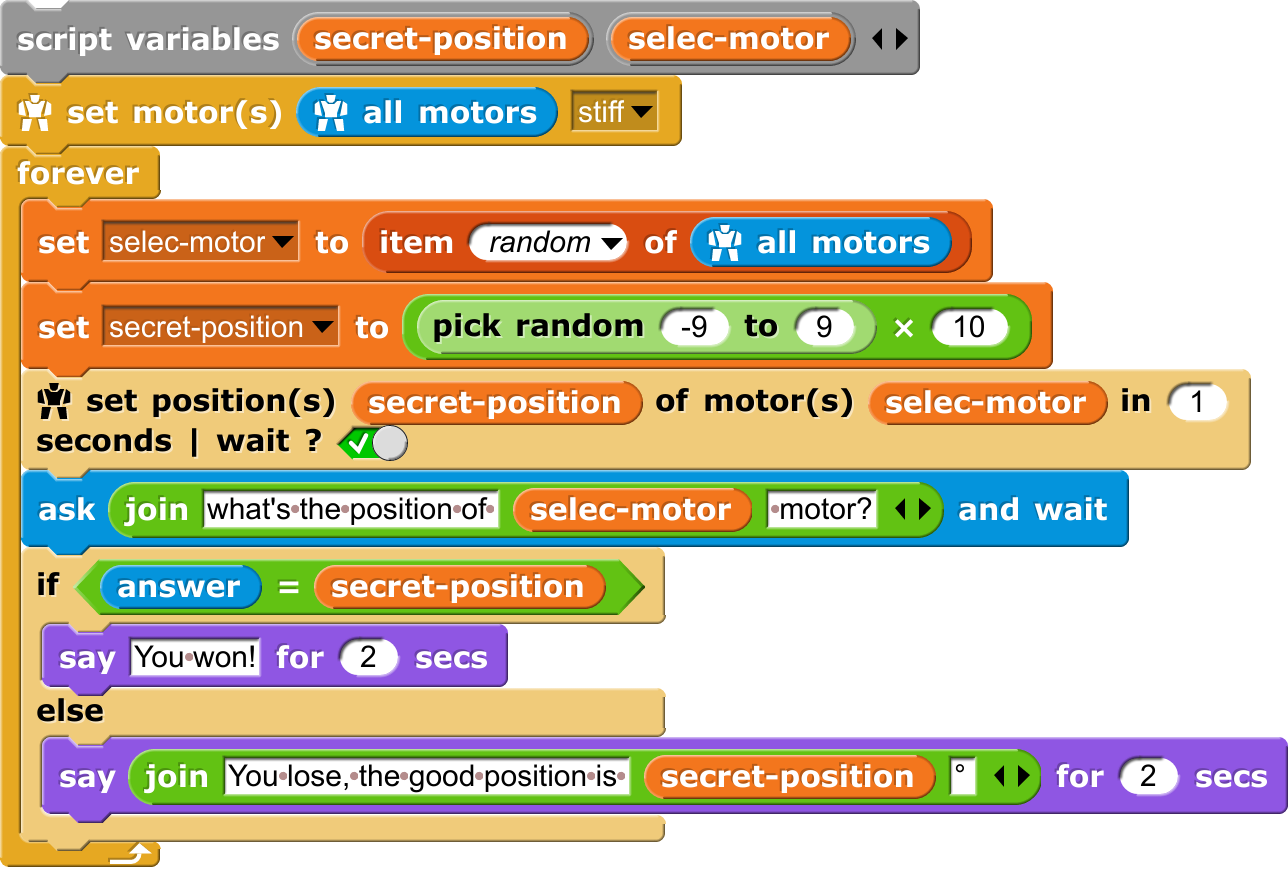
\includegraphics[width=0.9\linewidth]{Figures/prog-find_pos.png}
            \subcaption{Bloc de démonstration - Trouve la bonne position}\label{cod:prog_find_pos}
        \end{minipage}
        \strut\newline
        \begin{minipage}{\linewidth}
            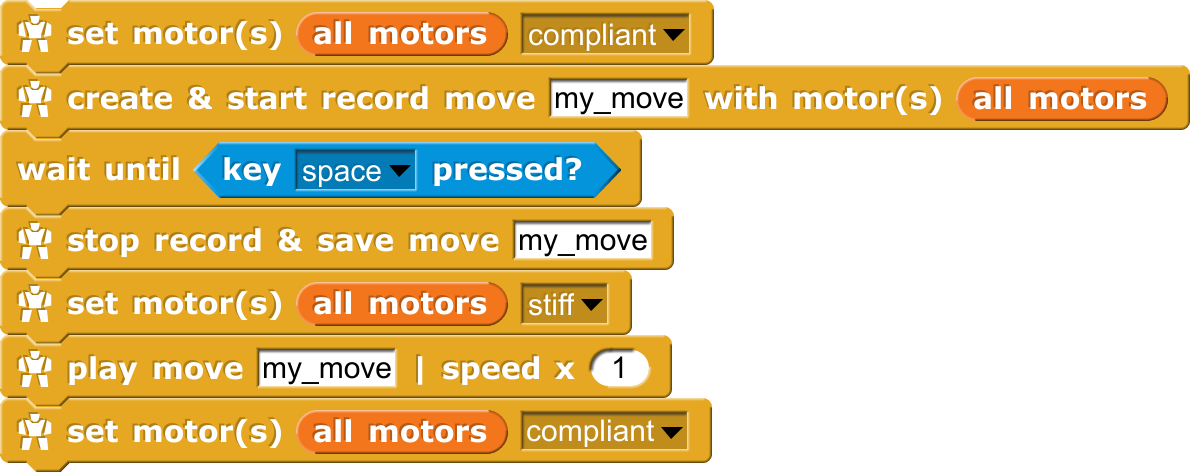
\includegraphics[width=0.9\linewidth]{Figures/prog-mime.png}
            \subcaption{Bloc de démonstration - Le Mime}\label{cod:prog_mime}
        \end{minipage}
        \caption{Bloc de démonstration \textit{Snap!}}
        \end{code}\par%
        \begin{code}
            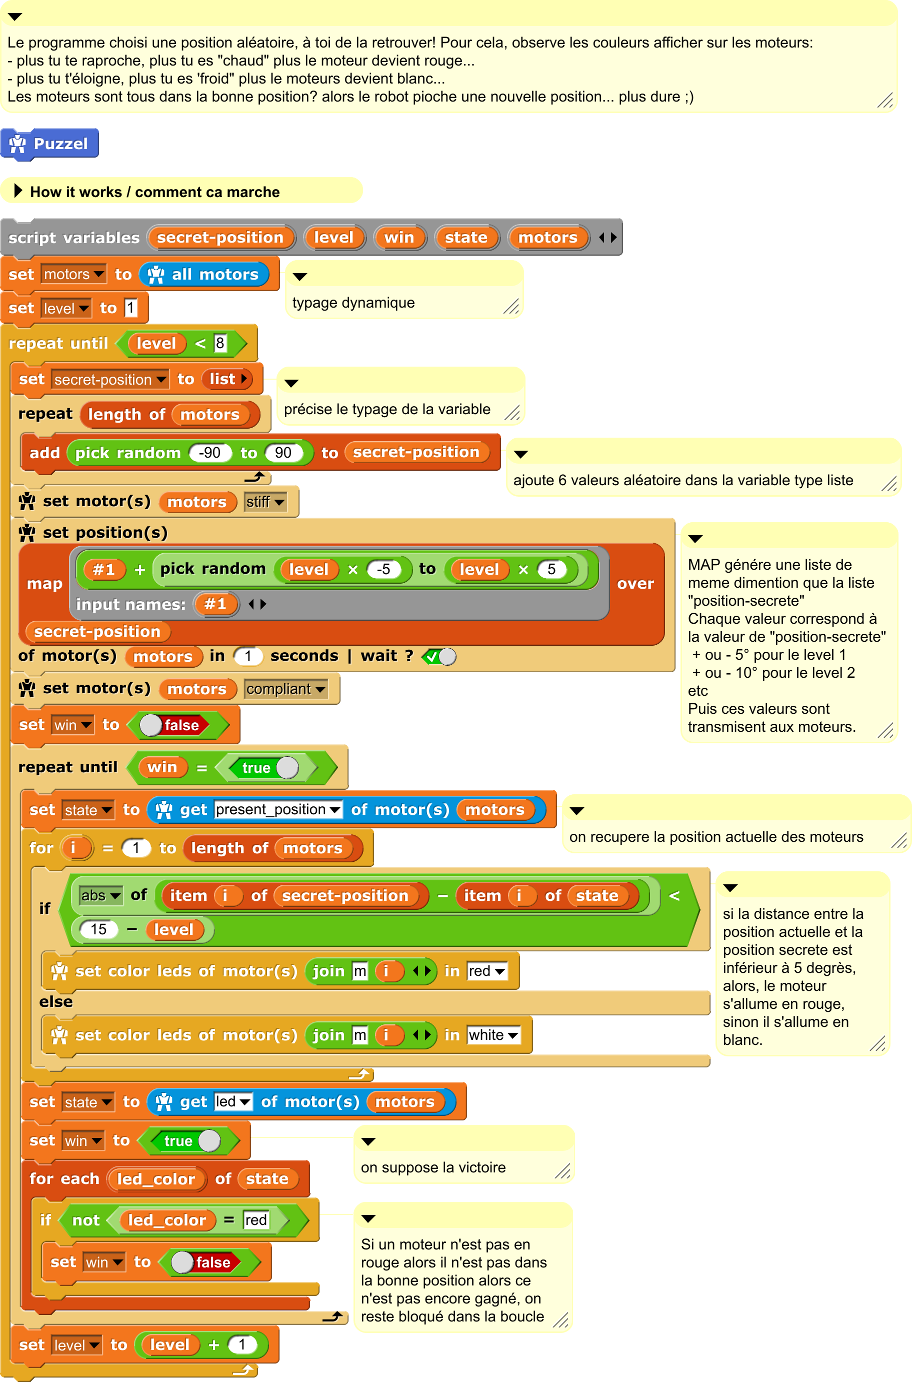
\includegraphics[width=0.85\linewidth]{Figures/prog-puzzle.png}
            \caption{Bloc de démonstration - Puzzle}\label{cod:prog_puzzle}
        \end{code}\par%
        \subsubsection{Activité en python}
            \paragraph{Les primitives}\label{sec:primitives}
                Les primitives correspondent à des programmes pré-enregistrés sur le robot. Un système d'orchestration fourni avec la bibliothèque PYPOT permet de les associer, de les synchroniser pour organiser des comportements complexes. Elles sont exécutées sous forme de thread et s'attachent au démarrage à l'instance du robot.
                Une primitive possède une phase courante (qui boucle), une phase  \cro{up} (au lancement) et une phase  \cro{down} (à sa fin). L’utilisateur peut rédiger et intégrer ses propres primitives qui seront alors disponibles (entre autres) dans  \cro{Poppy Monitor}.
            \paragraph{Les tutoriels notebook}
                Pour guider l'utilisateur dans la construction de ses programmes plusieurs exemples et tutoriels sont fournis~\citeURL{poppy-starter}. Cependant, la majorité des enseignants que nous avons suivie s'est principalement focalisée sur de la programmation visuelle avec \glsdesc{snap} ou sur des langages et des procédures qu'elle manipulait déjà. Seul, Georges Saliba a fourni plusieurs ressources en python, notamment un \sht{TD} de découverte~\citeURL{GS-TutoPython}, associé à un mini défi~\citeURL{GS-Python}. Il a également développé un tutoriel autour de la détection des QRcode par le robot~\citeURL{GS-QRcode}. De notre côté, nous avons développé un \sht{TD} permettant de découvrir les primitives et leur construction liées au \textit{Classe Object} et \textit{Héritage de Classe} en Python~\citeURL{TD-primitives}.
\begin{code}
\begin{lstlisting}[language=Python,basicstyle=\footnotesize]
def run(self):#on définit la fonction run()
    while not self.should_stop(): #tant que l'on ne demande pas d'arrêter
        for color in self.colors: #pour chacune des couleurs
            if not self.should_stop(): #si l'on ne demande pas d'arrêter
                if self.should_pause(): #si on me demande pause
                    self.wait_to_resume() #j'attends jusqu'à reprise
                for m in self.robot.motors: #pour chaque moteur
                    m.led = color #mettre la led dans la couleur
                for i in range(5):
                #je vérifie dix fois par période si l'on ne demande pas d'arrêter la primitives
                    if not self.should_stop():
                        if self.should_pause(): 
                            self.wait_to_resume()
                        time.sleep((1./self.freq)/5)
\end{lstlisting}
\caption[Exemple de Primitives (Tinsel, pyhon)]{\label{cod:tinsel}Extrait de la primitive Tinsel \citeA{pdf:demo.py}: fontion run()}
\end{code}\par%
            \paragraph{En forte progression}
                Depuis l'arrivée de l'option \sht{NSI}~\citeS{sec:ref_2019}, qui offre un nombre d'heures conséquent à la programmation et à l'apprentissage de leurs paradigmes, nous observons que de plus en plus d'enseignants s'informent et développent leurs compétences dans ce domainerge. Ceci amènera sans doute à la création de nouveaux contenus.
    \subsection{Autres exemples}
        \paragraph[Des robots anthropomorphes]{Des robots anthropomorphes}
            Bien que plus compliquées à mettre en place, notamment à cause de leur coût pour les établissements scolaires, les activités avec la plateforme Poppy Humanoïde et Poppy Torso sont riches de nombreux enseignements.
            \subparagraph{École Primaire}
                Nous pouvons notamment citer les retours d'expériences avec les élèves du premier et deuxième cycle:  La fascination qu'ils semblent éprouver à la vue de cette machine de même taille qu'eux, nous a permis d'aborder des questions fondamentales sur la constitution des corps et des êtres. En cherchant les différences et les similitudes entre eux et le robot (muscle/moteur; énergie électrique/nourriture; capteur/sens; \etc) nous avons pu démystifier ces machines et poser les premières bases pour développer un regard objectif et critique sur celles-ci. Mais ceci semble également leur avoir permis d'acquérir une meilleure perception de leur propre corps et de leurs capacités.
            \subparagraph{Licence 2\ieme année Danse}\label{sec:villard_cours}
                Toujours avec les plateformes anthropomorphes, un exemple avec Marie-Aline Villard, une enseignante-chercheuse en danse, ayant utilisé là le Poppy Humanoïde avec des étudiantes de 2ème année de licence de danse~\citeURL{MV-danse}. La majorité de ces étudiantes souhaite, après leurs études, pratiquer une activité d'enseignement. Ainsi M-A Villard a mis en place une série de séances où le mouvement était pensé à travers le robot. Voir les contraintes et les limites des articulations et moteurs propres au robot est différent de leurs propres contraintes  \cro{les aider à mieux appréhender le corps de l'autre}; chose qui leur sera essentielle quand il s'agira d'enseigner des mouvements de danse à leurs propres élèves. Mais ce travail est allé beaucoup plus loin et a donné lieu à une publication dans la revue IRIS (revue du centre de recherche sur l'imaginaire de Grenoble) à l'automne 2015~\citeB{villard2016mouv}.
            \subparagraph{Ensam Bordeaux}
                Un autre projet mettant en jeu ces robots est le concours Poppy proposé aux étudiants de l'ENSAM dans le cadre du diplôme bachelor. Ici les robots Torso sont utilisés comme briques technologiques à optimiser afin de répondre à un cahier des charges. La première année, les étudiants devaient développer un système de main préhenseur à adapter au robot~\citeURL{torso-hand}. La seconde année ils devaient concevoir une plateforme mobile pour le robot~\citeURL{torso-spot}. Aujourd'hui c'est un véritable fil rouge qui est utilisé.
            \subparagraph{École privé, Dassault Systeme}
                Nous pouvons également noter la démarche de la 3DS academy ciblant un public assez similaire, mais qui leur propose un parcours tutoré complet constitué comme un MOOC, plutôt que d'appliquer une démarche de projet \etou de concours~\citeURL{3DS-ac}.
\section{Limites}
    Plusieurs éléments nous ont limités dans la constitution des ressources pédagogiques. D'une part car l'objectif principal était de répondre aux besoins et aux contraintes des enseignants par rapports aux prescriptions officielles sur l'enseignement qu'ils avaient à réaliser. Et d'autre par, car chaque enseignant possède une expérience et une formation initiale qui lui est propre. Ainsi, les orientations qu'il donne à ses ressources sont tout autant personnelles et adaptées à son propre public (sa classe, possédant également ses propres spécifications). Dès lors, nous pouvons souligner que la majorité des enseignants, aujourd'hui en activité en France, n'ont pas eu (ou peu) de formation dans les domaines du numérique au cours de leur cursus scolaire. 
    De plus, il existe aujourd'hui une offre limitée concernant la formation continue sur ces sujets~\citeS{sec:formation}. En revanche, la majorité des élèves, étant  \cro{nés dedans}, ont une fausse impression de connaissance. De ces deux états de faits, émerge une réelle complexité à enseigner le numérique. 
    L'enseignant doit, d'une part, monter en compétence et d'autre part, savoir détecter les fausses connaissances que les élèves ont pu acquérir durant leurs expériences préalables avec le numérique et la robotique. Pour cela, il est nécessaire que l'enseignant ait une réelle appropriation des concepts qu'il manipule ainsi que des plateformes qu'il utilise pour illustrer ces concepts. 
    Ceci explique pour grande partie, pourquoi aujourd'hui la majorité des ressources pédagogiques se concentrent sur l'appropriation des concepts élémentaires de programmation via l'utilisation de langages de programmation visuels. Mais de nombreux exemples \tiret{pour certains cités dans ce manuscrit} ont montré la possibilité d'approfondir ces activités, notamment vers des concepts liés à l'\sht{IA}.